\chapter{طراحی جاذب دینامیکی ارتعاش سیستم کاهش مرتبه یافته 2 درجه آزادی به کمک الگوریتم ژنتیک }
\subsubsection{پارامترهای سامانه بنچمارک}

به‌منظور ارزیابی اثربخشی الگوریتم \lr{GA} معرفی‌شده بر روی معیار تکین (\lr{singular criterion})، یک تحلیل عددی با استفاده از مقادیر دلخواه برای سامانه کاهش یافته اصلی انجام شد. مقادیر به‌کاررفته در جدول~\ref{tab:benchmark-main-params} آمده‌اند.

\begin{table}[h!]
\centering
\caption{مقادیر پارامترهای سامانه اصلی در مثال بنچمارک}
\label{tab:benchmark-main-params}
\begin{tabular}{lc}
\hline
\textbf{پارامتر} & \textbf{مقدار} \\
\hline
$\Lambda$ & $1$ \\
$N$ & $1$ \\
$A_{\mathrm{Up}} = A_{\mathrm{Low}}$ & $0.0001$ \\
$F$ & $100$ \\
$\omega_{dc}$ & $1000$ \\
$\zeta_{dc}$ & $0.01$ \\
\hline
\end{tabular}
\end{table}

مقادیر هدف و وزن‌های متناظر برای این مثال بنچمارک به‌صورت زیر در نظر گرفته شده‌اند: پهنای‌باند هدف برابر با $1000~\text{rad/s}$ با وزن $0.30$؛ موقعیت قله‌های سامانه اولیه در $1000~\mtext{rad/s}$ و $2000~\mtext{rad/s}$ با وزن‌های جداگانه $0.35$ برای هر یک. این تنظیمات فرایند بهینه‌سازی را به‌سوی تعادلی میان پاسخ فرکانسی و کاهش دامنه هدایت می‌کند. وزن جریمه تنکی برابر $\alpha = 0.0002$ در نظر گرفته شده است؛ بدین معنا که امتیاز برازندگی متناسب با مجموع پارامترهای \lr{DVA} افزایش می‌یابد (همخوان با جزء \lr{L1} در رابطه‌ی \eqref{Eq.sparsity_penalty_detailed}). تلرانس هدف نیز برابر با $0.0012$ تثبیت شده است تا اطمینان دهد که حتی در بهترین حالت، همگرایی راه‌حل با تعداد محدودی از پارامترهای \lr{DVA} فعال رخ می‌دهد—اگرچه ممکن است به‌دلیل چالش‌های همگرایی یا عدم دسترس‌پذیری راه‌حل، این حالت دقیقاً حاصل نشود. با این حال، این راهبرد نشان می‌دهد چگونه می‌توان به بهترین بردار طراحی \lr{DVA} با کمترین تعداد پارامتر دست یافت. به‌طور خلاصه، این روش کارآمدی تابع برازندگی تعریف‌شده را تقویت می‌کند و موازنه (تریداف) شفافی میان اهداف مختلف طراحی \lr{DVA} برقرار می‌سازد.

\subsubsection{پیکربندی الگوریتم ژنتیک}

اهداف بهینه‌سازی به‌گونه‌ای انتخاب شده‌اند که عملکرد مطلوب را پاداش دهند و در عین حال از استفاده بیش‌ازحدِ مؤلفه‌های \lr{DVA} جلوگیری کنند. پهنای‌باند هدف $1000~\text{rad/s}$ با وزن $0.30$ و موقعیت قله‌های سامانه اولیه در $1000~\mtext{rad/s}$ و $2000~\text{rad/s}$ با وزن‌های $0.35$ برای هر یک در نظر گرفته شده‌اند (مطابق با ضرایب وزن $w_{ij}$ در \eqref{Eq.composite_measure_detailed}). برای ترغیب طرح‌های فشرده‌تر، جزء تنکی به تابع برازندگی افزوده می‌شود که به‌ازای هر پارامتر فعال \lr{DVA} (یا به‌طور کلی مجموع قدرمطلق پارامترها طبق \eqref{Eq.sparsity_penalty_detailed}) جریمه‌ای اعمال می‌کند. این چینش، جستجو را به‌سمت بهترین پاسخ فرکانسیِ قابل حصول با کمترین تعداد پارامتر سوق می‌دهد، از اجزای غیرضروری می‌کاهد و قابلیت پیاده‌سازی را بهبود می‌بخشد. در مواردی که قیود امکان‌پذیری یا مسائل همگرایی مانع رسیدن دقیق به مقادیر هدف شوند، چارچوب پیشنهادی همچنان «تنک‌ترین» راه‌حلِ با کارایی بالا را ترجیح می‌دهد.

\section{نتایج و بحث}
\subsection{پاسخ فرکانسی و پارامترهای بهینه \lr{DVA}}

پاسخ‌های \lr{FRF} جرمِ اصلی در دو حالت «بدون \lr{DVA}» و «با \lr{DVA} بهینه‌شده» در شکل \ref{fig:frf_comparison} نشان داده شده است. بازه فرکانسیِ بررسی‌شده از \(0\) تا \(2200\)\,\lr{Hz} امتداد دارد. در غیاب \lr{DVA}، یک قله رزونانسِ واحد در بازه \(1000\)\,\lr{Hz} تا \(2000\)\,\lr{Hz} مشاهده می‌شود که با الزامات «باندِ اجتناب» سازگار نیست. در مقابل، با افزودن \lr{DVA} بهینه، دو قله در مجاورتِ \(1000\)\,\lr{Hz} و \(2000\)\,\lr{Hz} قرار می‌گیرند و درونِ این باند، قله رزونانسی شکل نمی‌گیرد. بیرون از بازه \(1000\)\,\lr{Hz} تا \(2000\)\,\lr{Hz}، سطوح پاسخ در دو حالت مشابه و کوچک باقی می‌مانند.

\begin{figure}[htbp]
  \centering
  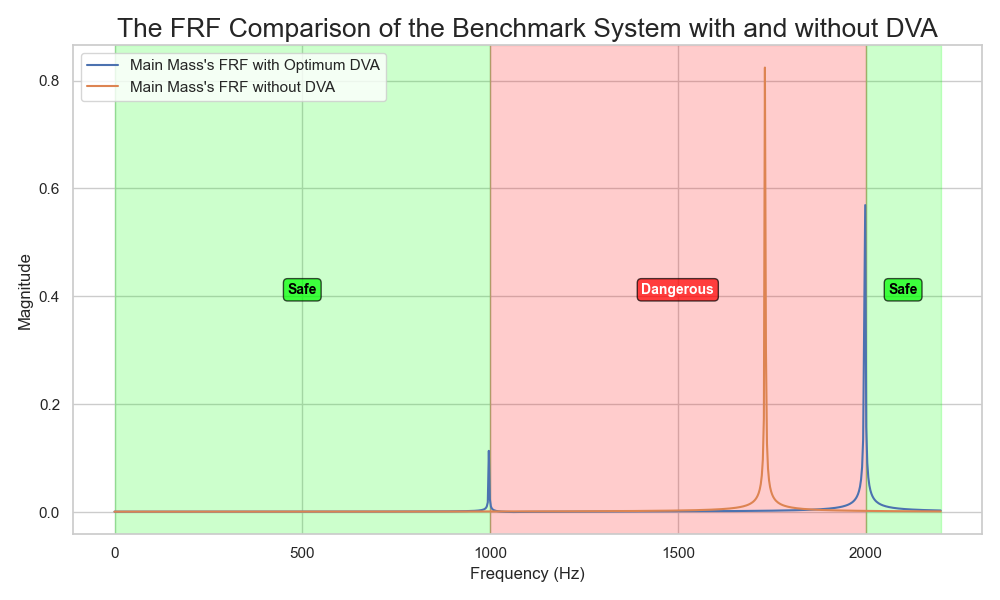
\includegraphics[width=\linewidth]{picture11.png}%
  \caption{پاسخ فرکانسیِ جرمِ اصلی در حالتِ بدون \lr{DVA} و با \lr{DVA} بهینه‌شده در بازه \lr{0–2200 Hz}. در حضور \lr{DVA} بهینه، دو قله در مجاورتِ \lr{1000 Hz} و \lr{2000 Hz} شکل می‌گیرد و درونِ باندِ اجتناب قله رزونانس مشاهده نمی‌شود.}
  \label{fig:frf_comparison}
\end{figure}

برای این مطالعه، باندِ اجتناب \(1000\)\,\lr{Hz} تا \(2000\)\,\lr{Hz} پیشاپیش تعیین شده بود. با \lr{DVA} بهینه، رزونانس‌ها درونِ این باند حذف شده‌اند و قله‌های غالب در لبه‌های باند مستقر شده‌اند؛ بدین‌ترتیب پهنای‌باندِ هدف حفاظت شده و نیازمندیِ طراحی با کمترین بزرگ‌نماییِ درون‌باندی برآورده گردیده است. این جایگذاریِ قله‌ها در مرزهای باند، ضمن حفظ رفتار خارج از باند، از برانگیختگی‌های ناخواسته در میانه باند جلوگیری می‌کند و نشان می‌دهد که سازوکارِ شکل‌دهیِ قله/ضدقله به‌صورت مؤثر به کار افتاده است.

\paragraph{بردار پارامترهای بهینه}
مجموعه پارامترهای بهینه \lr{DVA} به‌صورت زیر به‌دست آمد:
\[
\begin{aligned}
&\beta_1 = 0.0152,\quad \beta_7 = 0.5509,\quad \beta_8 = 0,\\
&\lambda_1 = 0.8235,\quad \lambda_7 = 0.2580,\quad \lambda_8 = 0.0789,\\
&\mu_1 = 0.3671,\quad \nu_1 = 0,\quad \nu_7 = 0,\quad \nu_8 = 0.
\end{aligned}
\]
صفر بودنِ مقادیرِ \(\nu\)‌ها بیانگر آن است که این کوپلینگ‌های میراکننده در راه‌حلِ بهینه لازم نبوده‌اند؛ در نتیجه پیکربندیِ تنک و کارآمدی حاصل شده که تنها مؤلفه‌های ضروری را فعال نگاه می‌دارد. از منظرِ پیاده‌سازی، این امر به معنای کاهشِ اجزای لازم، ساده‌تر شدنِ مونتاژ و نگهداشت، و کاهشِ حساسیت به عدم‌قطعیت‌های عملی است؛ در حالی‌که معیارهای عملکردیِ هدف نیز تأمین می‌شوند.

\paragraph{همگراییِ \lr{GA} و تحلیلِ برازندگی}
در شکل \ref{fig:ga_convergence}، بهترین و میانگینِ مقادیرِ برازندگی در طولِ \(500\) نسل گزارش شده‌اند. مقدار «بهترینِ اولیه» برابر با \(0.042936\) و «بهترینِ نهایی» برابر با \(0.001206\) است که بهبودِ مطلقِ \(0.041730\) را نشان می‌دهد. میانگینِ برازندگی کاهشِ سریعی در نسل‌های نخست دارد و سپس پیرامونِ بازه \(0.01\) تا \(0.02\) با نوساناتِ گهگاه (\lr{spikes}) نوسان می‌کند؛ در عین حال «بهترینِ برازندگی» پس از چند ده نسل به پوشِ پایینی نزدیک می‌ماند. این افتِ تندِ آغازین، با اکتشافِ خشنِ مؤثرِ \lr{GA} سازگار است و شکافِ پایدار میان «میانگین» و «بهترین» نشان می‌دهد که تنوعِ جمعیت در طولِ جستجو حفظ شده است؛ هر دو ویژگی برای اجتناب از گیر افتادن در کمینه‌های محلی اهمیت دارند.

\begin{figure}[htbp]
  \centering
  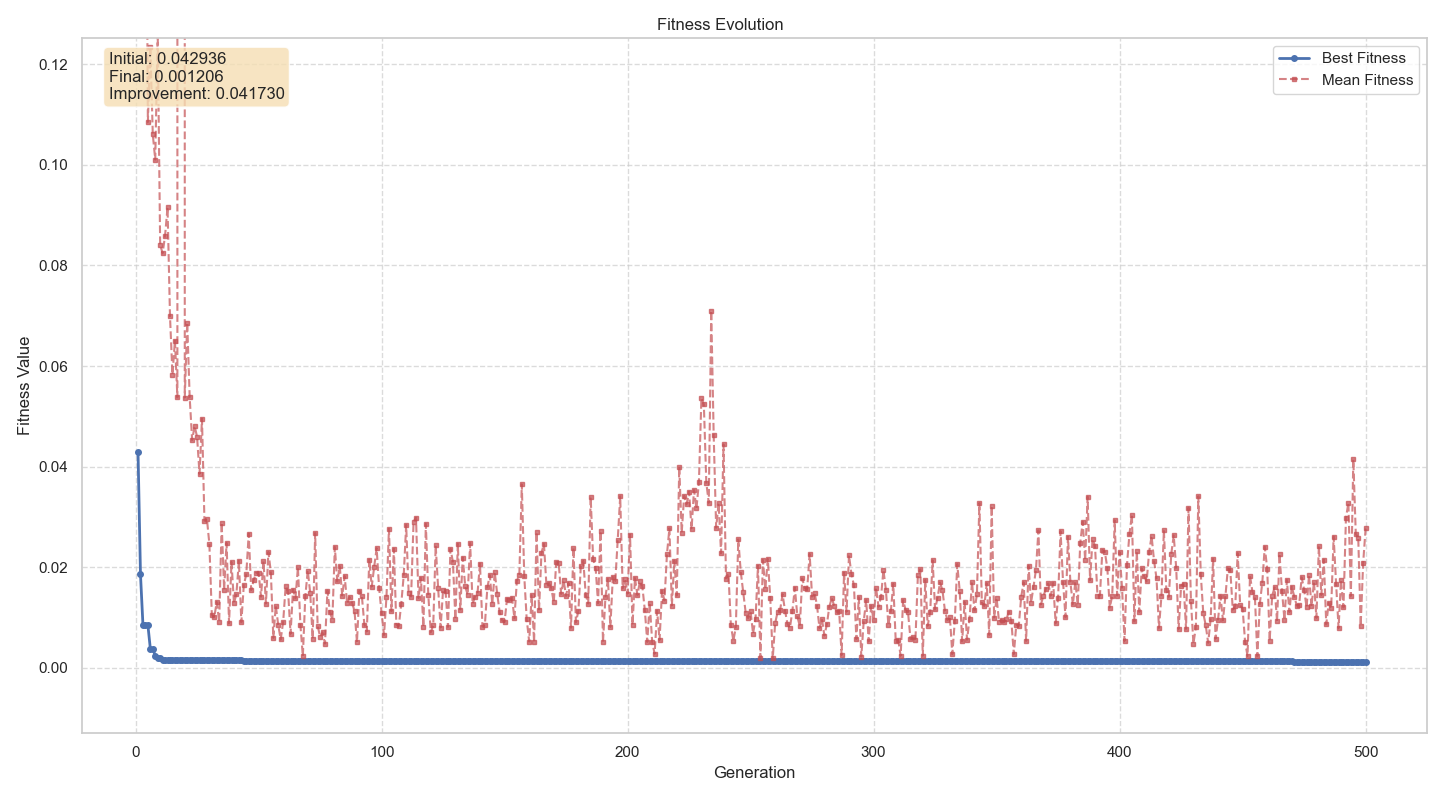
\includegraphics[width=\linewidth]{picture12.png}%
  \caption{روندِ همگراییِ الگوریتمِ ژنتیک: بهترین و میانگینِ برازندگی در طولِ \lr{500} نسل. بهترینِ برازندگی از \lr{0.042936} به \lr{0.001206} کاهش یافته است و شکافِ پایدار میان «میانگین» و «بهترین» نشان‌دهنده حفظِ تنوعِ جمعیت است.}
  \label{fig:ga_convergence}
\end{figure}

مقدارِ کلِ تابعِ هدف در حالتِ نهایی \(f=0.001206\) است که به‌صورتِ سهم‌های زیر ترکیب شده است: \(40.8\%\) از مؤلفه هدفِ اصلی، \(34.7\%\) از جریمه تنکی، و \(24.5\%\) از مؤلفه خطایِ درصدی (مطابق شکل \ref{fig:objective_breakdown}). این تجزیه وزنی نشان می‌دهد که ضمن تحققِ معیارِ اولیه عملکرد (شکل‌دهیِ قله‌ها و کنترلِ درون‌باند)، سازوکارِ تنک‌سازی نقشِ قابل‌توجهی در هدایتِ راه‌حل به سوی پیکربندی‌های کم‌مایه‌تر ایفا کرده و مؤلفه خطایِ درصدی نیز به ریزتنظیمِ معیارهای جزئی (نظیر پهنای‌باندِ مؤثر، شیبِ محلی و مساحتِ زیرِ منحنی) کمک کرده است.

\begin{figure}[htbp]
  \centering
  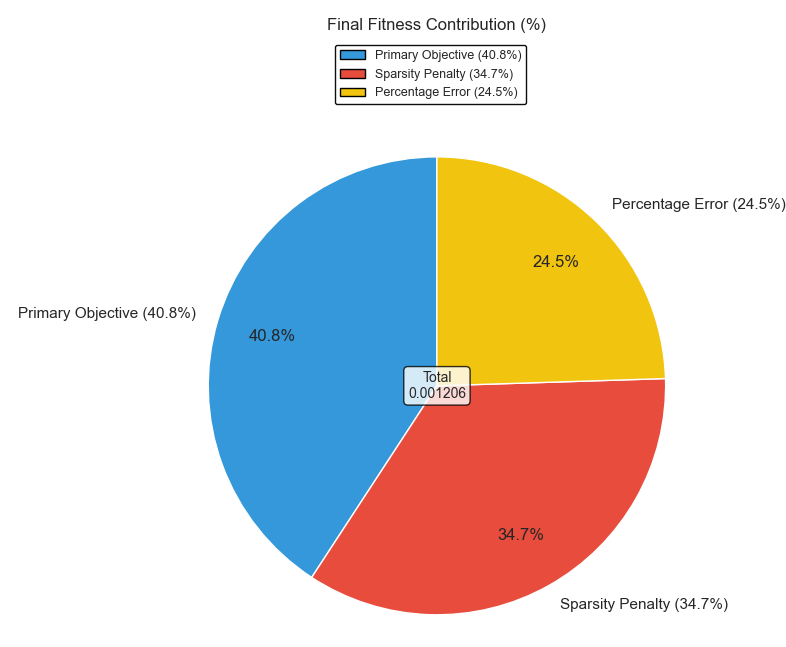
\includegraphics[width=0.9\linewidth]{picture13.png}%
  \caption{تفکیکِ سهمِ مؤلفه‌هایِ تابعِ هدف در مقدارِ نهایی \(f=0.001206\): مؤلفه هدفِ اصلی \lr{40.8\%}، جریمه تنکی \lr{34.7\%}، و مؤلفه خطایِ درصدی \lr{24.5\%}.}
  \label{fig:objective_breakdown}
\end{figure}

در مجموع، نتایج نشان می‌دهند که چارچوبِ بهینه‌سازیِ مبتنی بر \lr{GA} و تابعِ هدفِ تعریف‌شده قادر است باندِ اجتناب \(1000\)\,\lr{Hz} تا \(2000\)\,\lr{Hz} را بدونِ قله درون‌باندی حفظ کند، قله‌هایِ اصلی را در لبه‌هایِ باند جای دهد، و در عینِ حال با تکیه بر جریمه تنکی، به راه‌حل‌هایی با حداقلِ مؤلفه‌هایِ فعال دست یابد. این توازن، همخوان با نیازهایِ طراحیِ عملیِ \lr{DVA}، میانِ «عملکردِ فرکانسیِ مطلوب» و «پیاده‌سازیِ ساده و پایا» برقرار می‌کند.


% پیش‌نیازهای پیشنهادی در پرامبل:
% \usepackage{graphicx}
% \usepackage{caption}        % برای \ContinuedFloat
% \usepackage{subcaption}     % در صورت نیاز به زیرفضای شرح (اینجا از \ContinuedFloat استفاده شده است)
% \captionsetup{font=small}

\subsection{نقش جریمه تنکی و تحلیل روندها}

سهم قابل توجهِ جزءِ جریمه تنکی در طول بهینه‌سازی مشهود است، با این حال مقدار نهایی کوچک باقی می‌ماند؛ این موضوع نشان می‌دهد که هدفِ اصلی بدون اتکا به تعداد زیادی متغیرِ تنظیم به دست آمده است. مقادیر نزدیک به صفرِ منتسب به اکثر پارامترها دلالت دارد که تنها یک زیرمجموعه حداقلی برای برآوردن اهداف کافی بوده است؛ امری که با پیکربندیِ \emph{کم‌مایه و پارسیمون} \lr{DVA} ــ با پرهیز از مؤلفه‌های غیرضروری ــ سازگار است.

\paragraph{نرخ بهبود به‌ازای هر نسل}
در شکل \ref{fig:improvement_rate}، نرخ بهبودِ به‌ازای هر نسل برای تمامِ \(500\) نسل ترسیم شده است. قله‌های بزرگ به فاز آغازین محدود می‌شوند و پس از آن نرخ به سمت صفر میل می‌کند و تنها افزایش‌های کوچک و پراکنده مشاهده می‌شود. میانگینِ نرخ بهبود، برابر با \(8.4\times 10^{-5}\) به‌ازای هر نسل نشانه‌گذاری شده است. بهبودهای سریع در نسل‌های ابتدایی متمرکزند و سپس تغییرات رو به کاهش می‌گذارند؛ رفتاری که با همگرایی به یک بهینه پایدار سازگار است. نرخ‌های نزدیک به صفر در بخش پایانیِ اجرا نشان می‌دهد که صرفاً اصلاحاتِ محلیِ کوچک رخ داده و راه‌حل عملاً پایدار شده است.

\begin{figure}[htbp]
  \centering
  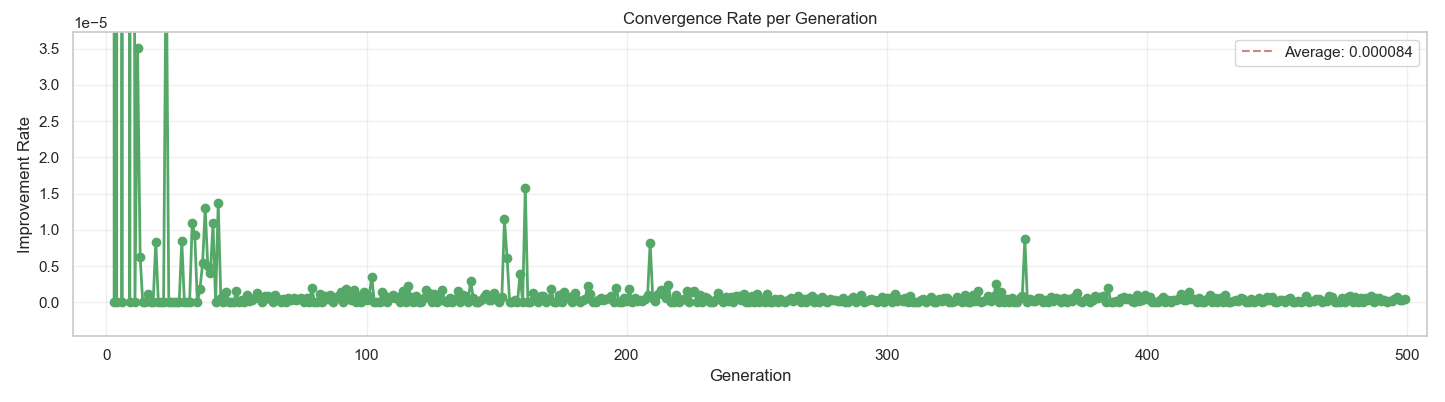
\includegraphics[width=\linewidth]{picture14.png}%
  \caption{نرخ بهبودِ به‌ازای هر نسل در طول \(500\) نسل. قله‌های بزرگ در فاز آغازین مشاهده می‌شوند و سپس نرخ بهبود به مقادیر نزدیک به صفر می‌رسد؛ میانگین نرخ بهبود \(8.4\times 10^{-5}\) به‌ازای هر نسل است.}
  \label{fig:improvement_rate}
\end{figure}

\paragraph{روند همگراییِ \(\mu_1\)}
در شکل \ref{fig:mu1_convergence}، پارامتر \(\mu_1\) طی \(500\) نسل رهگیری شده است. مقدار آغازین \(\mu_1=0.393887\) و مقدار نهایی در نسل پایانی \(\mu_1=0.367131\) ثبت شده است؛ یعنی کاهش خالص \(\,0.026756\). یک روند خطی با شیب \(-3.41\times 10^{-4}\) به‌ازای هر نسل برازش داده شده است. متوسط افزایشِ نسل‌به‌نسل \(-5.4\times 10^{-5}\) بوده است. گستره مشاهده‌شده \(0.2159\) و انحراف معیار \(0.0535\) گزارش شده‌اند. الگوی مشاهده‌شده نشان‌دهنده یک رانشِ کاهشیِ تدریجی با گام‌های کوچک و سپس پایدارسازی در نسل‌های متأخر است. همگرایی عمدتاً با رانشِ یکنواختِ کاهشی و کاهش اندازه گام‌ها کنترل شده است؛ نوساناتِ پایدار مشاهده نشد و مقدار نهایی به‌خوبی درون بازه مجاز قرار دارد، بنابراین \(\mu_1\) پارامتری فعال باقی می‌ماند.

\begin{figure}[htbp]
  \centering
  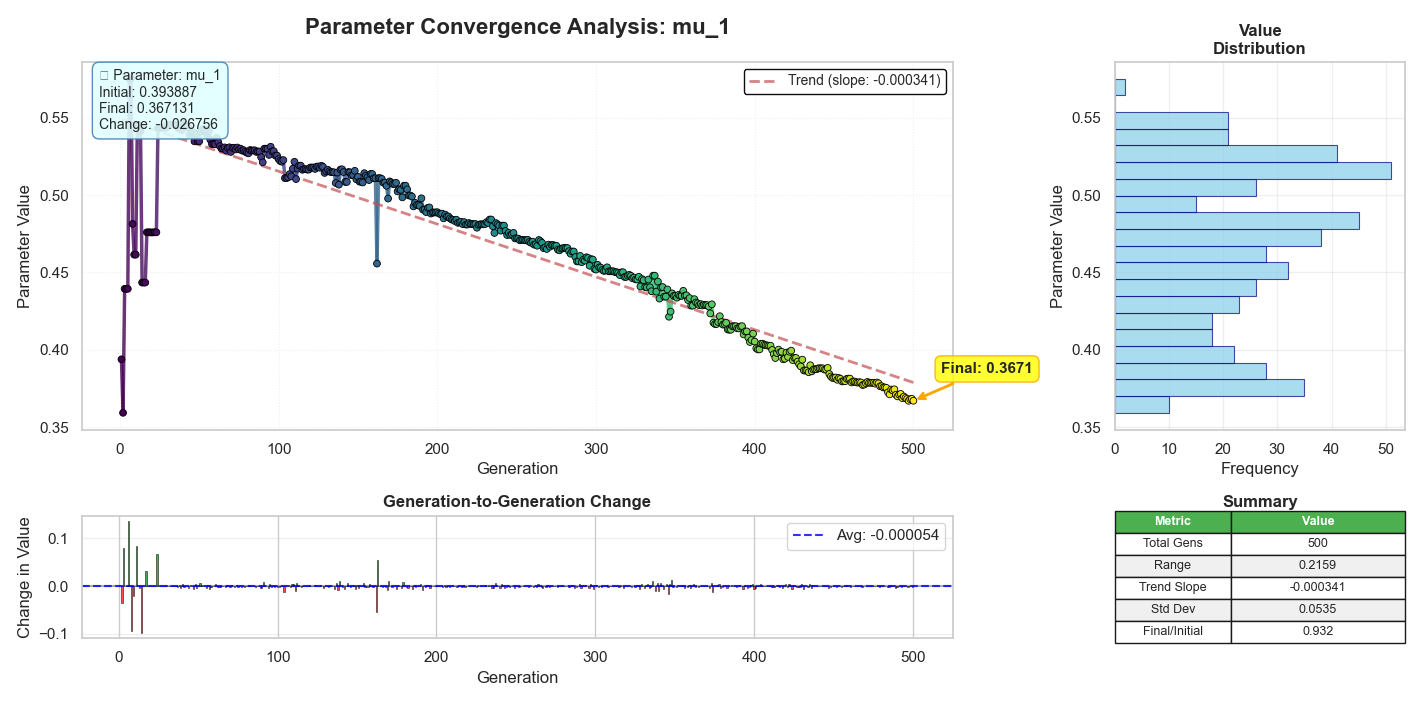
\includegraphics[width=\linewidth]{picture15.png}%
  \caption{همگراییِ \(\mu_1\) در طول \(500\) نسل: مقدار آغازین \(0.393887\)، مقدار نهایی \(0.367131\)، کاهش خالص \(0.026756\)، شیب روند خطی \(-3.41\times 10^{-4}\) به‌ازای هر نسل، میانگین افزایشِ نسل‌به‌نسل \(-5.4\times 10^{-5}\)، گستره \(0.2159\) و انحراف معیار \(0.0535\).}
  \label{fig:mu1_convergence}
\end{figure}

\paragraph{همگراییِ پارامترها به‌تفکیک}
جمع‌بندیِ همگراییِ پارامترها در شکل‌های \ref{fig:beta_convergence} تا \ref{fig:nu_convergence} آمده است: پارامترهای \(\beta\) در شکل \ref{fig:beta_convergence}، پارامترهای \(\lambda\) در شکل \ref{fig:lambda_convergence} و پارامترهای \(\nu\) در شکل \ref{fig:nu_convergence}. برای هر پارامتر، مسیرِ تکاملی در طول نسل‌ها همراه با توزیع مقدار و سنجه‌های خلاصه نمایش داده شده است. به‌منظور چیدمانِ عمودیِ پنل‌ها و امکان شکستِ خودکارِ محتوا روی چند صفحه، از چند \texttt{figure} با \texttt{\textbackslash ContinuedFloat} برای هر شماره‌شکل استفاده شده است.

% ===== Fig. 8: Convergence of beta parameters (a)(b)(c), vertically stacked with automatic page breaks =====
\begin{figure}[h]
  \centering
  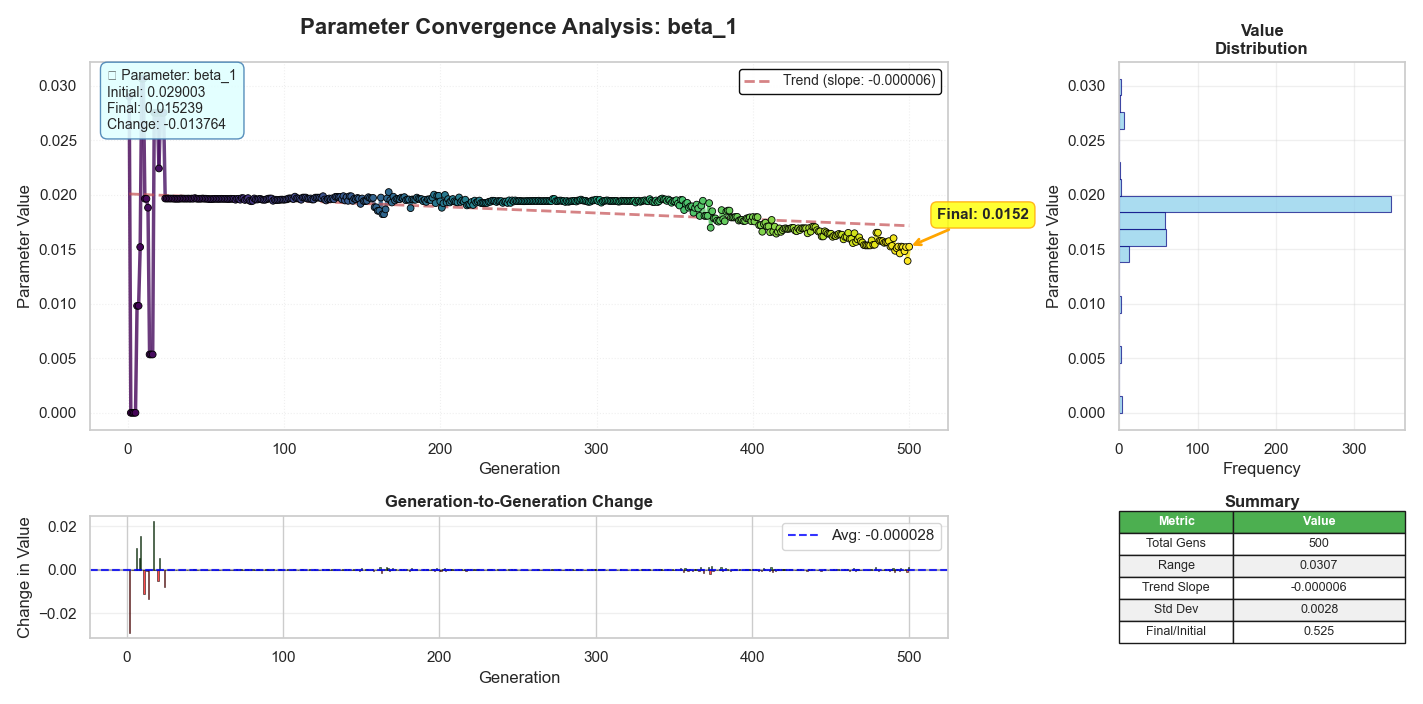
\includegraphics[width=\linewidth]{picture16.png}%
  \caption{همگراییِ پارامترهای \(\beta\): (a) \(\beta_1\).}
  \label{fig:beta_convergence}
\end{figure}

\begin{figure}[h]\ContinuedFloat
  \centering
  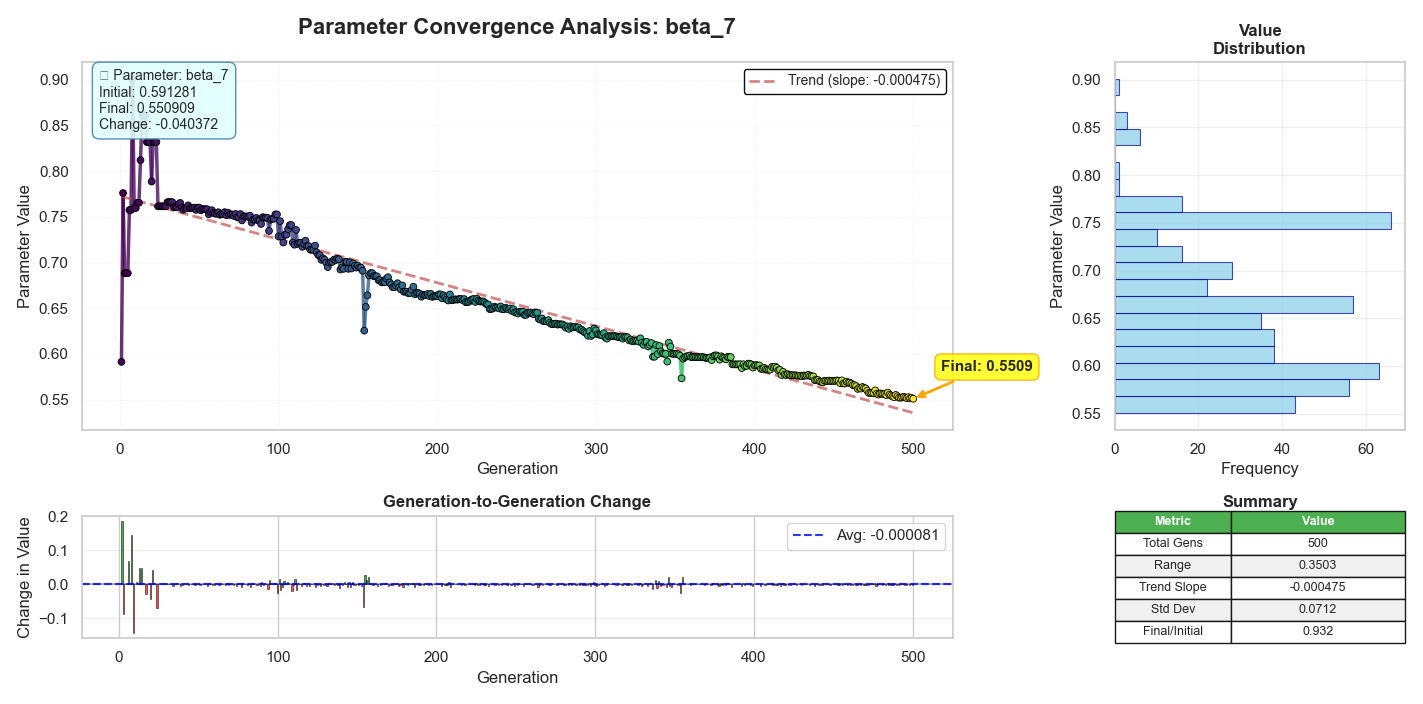
\includegraphics[width=\linewidth]{picture17.png}%
  \caption{(b) \(\beta_7\).}
\end{figure}

\begin{figure}[h]\ContinuedFloat
  \centering
  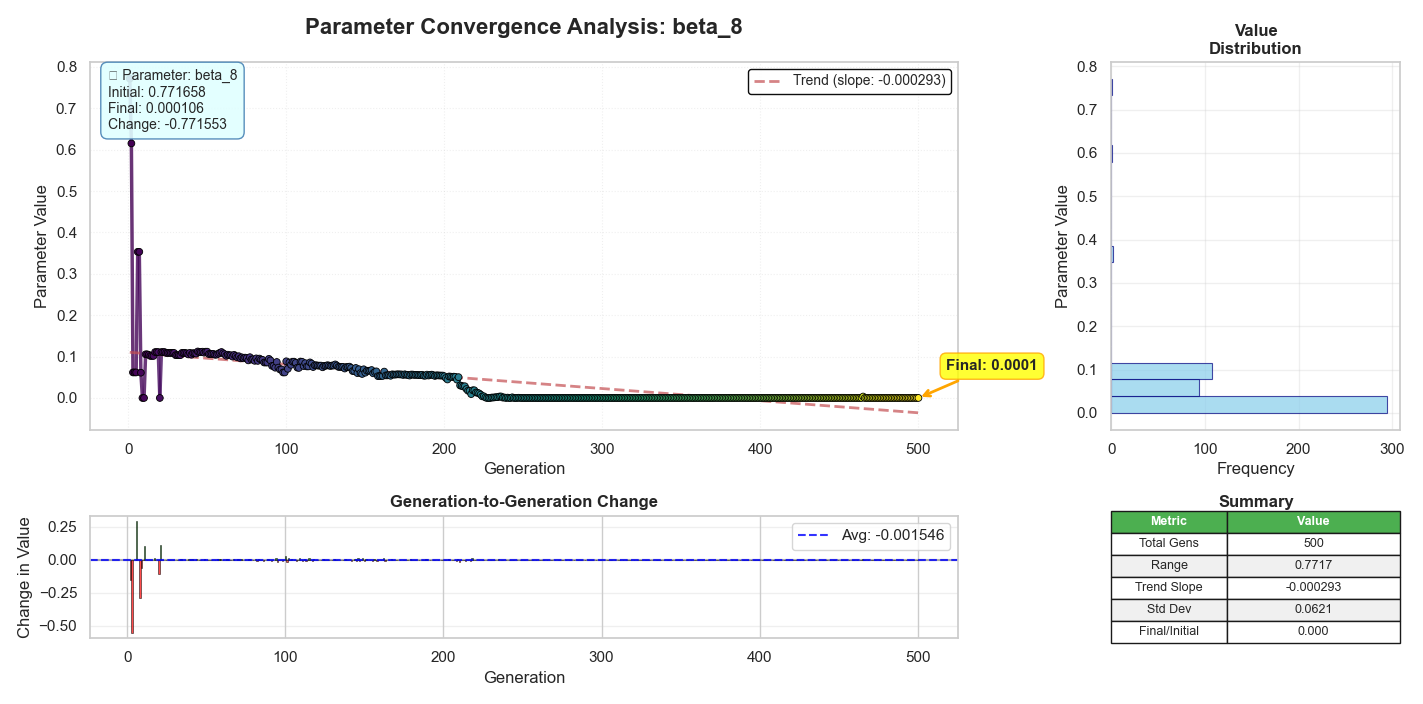
\includegraphics[width=\linewidth]{picture18.png}%
  \caption{(c) \(\beta_8\).}
\end{figure}

\paragraph{تحليل پارامترهاي \(\beta\) در شكل \ref{fig:beta_convergence}}

\textbf{بخش (a) — \(\beta_1\):}
در بخش (a) از شكل \ref{fig:beta_convergence}، \(\beta_1\) طي \(500\) نسل رهگيري شده است. مقدار آغازين \(\beta_1=0.029003\) و مقدار نهايي \(\beta_1=0.015239\) ثبت شده كه كاهش خالص \(\,0.013764\) را نشان مي‌دهد. روند خطي برازش‌شده داراي شيب \(-6.0\times 10^{-6}\) به‌ازاي هر نسل است و ميانگين افزايش نسل‌به‌نسل \(-2.8\times 10^{-5}\) گزارش شده است. بازه مشاهده‌شده \(0.0307\) و انحراف معيار \(0.0028\) است؛ توزيع مقادير باريك و حول \(0.019\) متمركز است. مسير تقريباً ثابت در ابتدا و سپس افت ملايم در مراحل انتهايي مشاهده مي‌شود. پايدارسازي درون ناحيه مجاز رخ داده است؛ از اين‌رو \(\beta_1\) در نقطه بهينه به‌عنوان يك متغير تنظيم كوچك اما «فعال» باقي مانده كه با تنظيمات دقيق (نه رفتار مرزي) سازگار است.

\medskip
\textbf{بخش (b) — \(\beta_7\):}
در بخش (b) از شكل \ref{fig:beta_convergence}، \(\beta_7\) از \(0.591281\) به \(0.550909\) تغيير كرده و تغيير خالص \(-0.040372\) را نشان مي‌دهد. روند خطي برازش‌شده داراي شيب \(-4.75\times 10^{-4}\) به‌ازاي هر نسل و ميانگين افزايش نسل‌به‌نسل \(-8.1\times 10^{-5}\) است. بازه اندازه‌گيري‌شده \(0.3503\) و انحراف معيار \(0.0712\) گزارش شده‌اند. يك رانش نزولي يکنواخت با كوچك‌شدن تدريجي گام‌ها مشاهده مي‌شود كه به پايدارسازي پايدار ختم مي‌گردد. اندازه نسبتاً بزرگ \(\beta_7\) نسبت به \(\beta_1\) حاكي از نقش اوليه \(\beta_7\) در شكل‌دهي پاسخ \lr{FRF} است.

\medskip
\textbf{بخش (c) — \(\beta_8\):}
در بخش (c) از شكل \ref{fig:beta_convergence}، \(\beta_8\) طي \(500\) نسل پايش شده است. مقدار آن از \(0.771658\) به \(0.000106\) رسيده و كاهش \(\,0.771553\) را نشان مي‌دهد. روند خطي برازش‌شده داراي شيب \(-2.93\times 10^{-4}\) به‌ازاي هر نسل و ميانگين افزايش نسل‌به‌نسل \(-0.001546\) است. بازه مشاهده‌شده \(0.7717\) و انحراف معيار \(0.0621\) گزارش شده‌اند. هيستوگرام نشان‌دهنده تراكم بالا در مقادير نزديك به صفر پس از نسل‌هاي ابتدايي است. يك فروپاشي سريعِ آغازين به سوي صفر مشاهده مي‌شود و پس از آن فقط اصلاحات ناچيز رخ مي‌دهد. مقدار نهاييِ نزديك به صفر بيان مي‌كند كه \(\beta_8\) عملاً توسط بهينه‌سازي هرس شده است؛ امري سازگار با هدف تنكي و پرهيز از متغيرهاي تنظيم غيرضروري.


% ===== Fig. 9: Convergence of lambda parameters (a)(b)(c), vertically stacked =====
\begin{figure}[h]
  \centering
  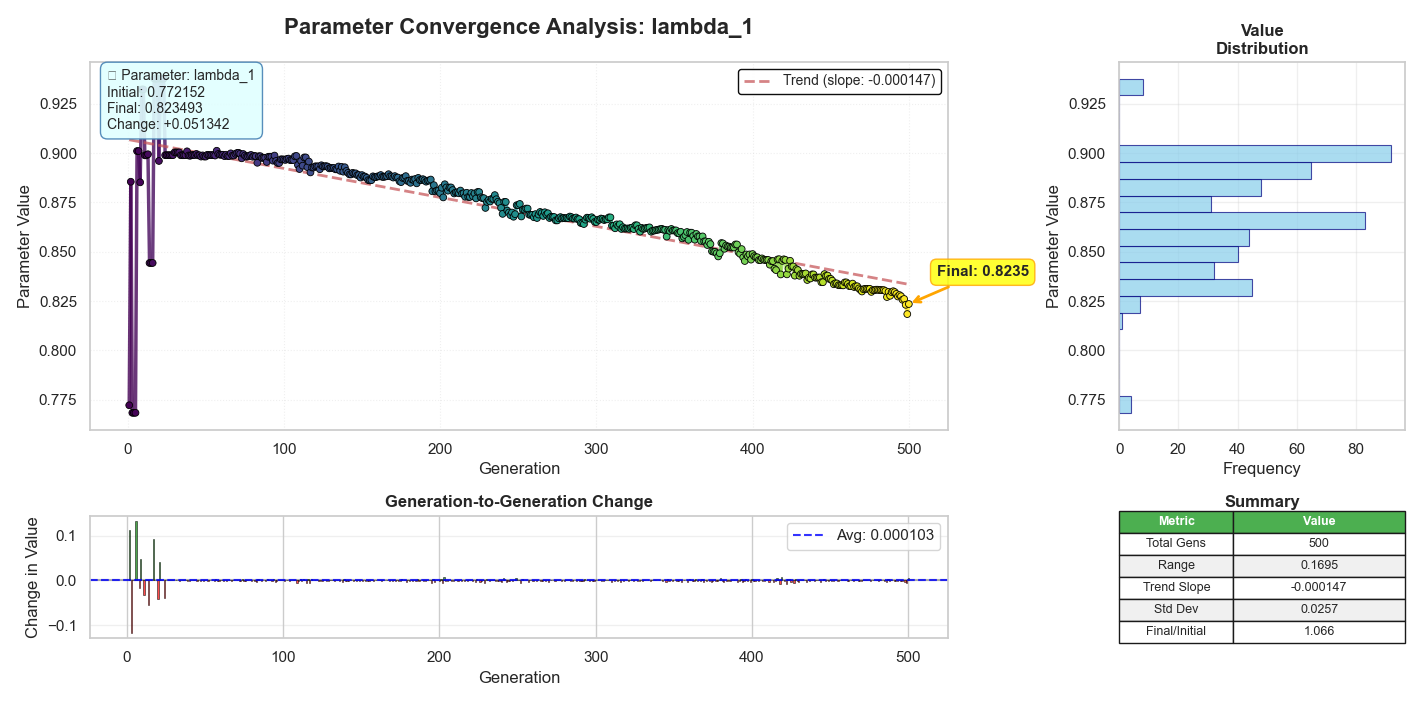
\includegraphics[width=\linewidth]{picture19.png}%
  \caption{همگراییِ پارامترهای \(\lambda\): (a) \(\lambda_1\).}
  \label{fig:lambda_convergence}
\end{figure}

\begin{figure}[h]\ContinuedFloat
  \centering
  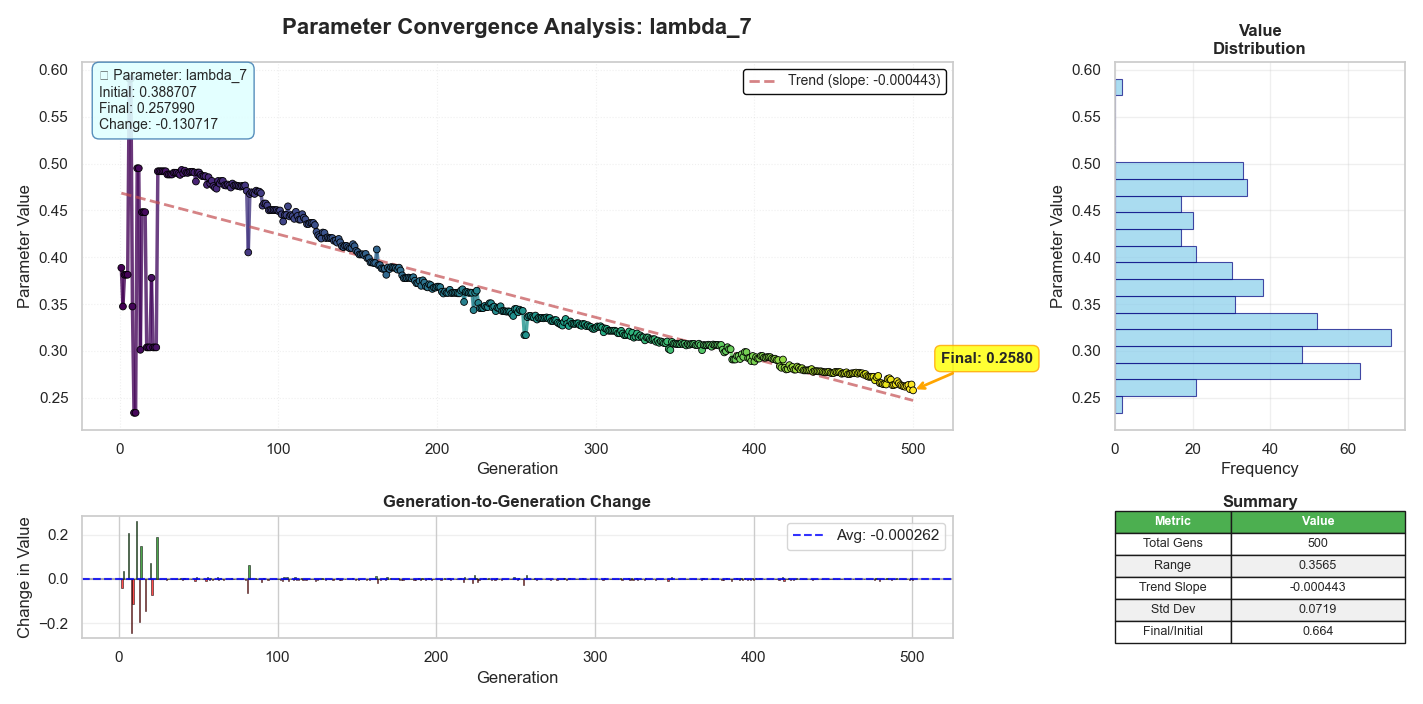
\includegraphics[width=\linewidth]{picture20.png}%
  \caption{(b) \(\lambda_7\).}
\end{figure}

\begin{figure}[h]\ContinuedFloat
  \centering
  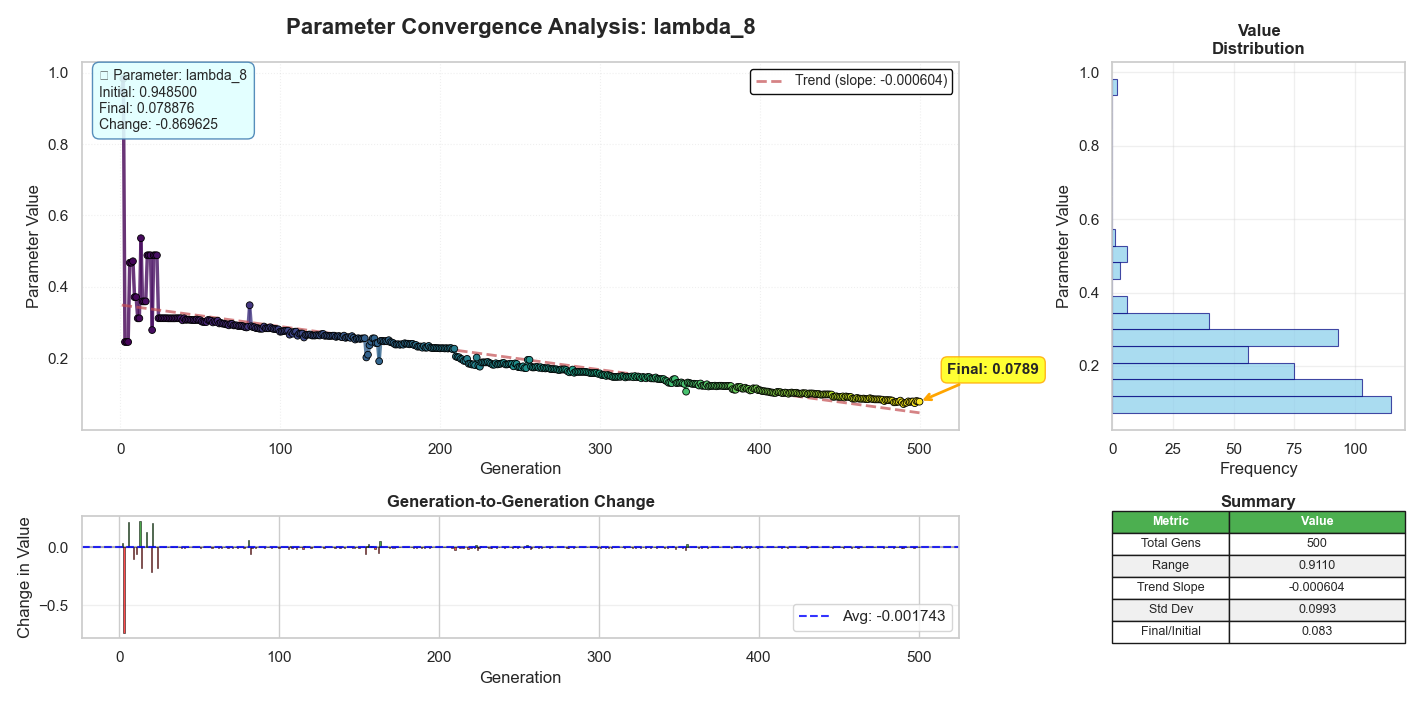
\includegraphics[width=\linewidth]{picture21.png}%
  \caption{(c) \(\lambda_8\).}
\end{figure}

\paragraph{تحلیل پارامترهای \(\lambda\) در شکل \ref{fig:lambda_convergence}}

\textbf{بخش (a) — \(\lambda_1\):}
در بخش (a) از شکل \ref{fig:lambda_convergence}، \(\lambda_1\) طی \(500\) نسل رهگیری شده است. مقدار آغازین \(\lambda_1=0.772152\) و مقدار نهایی \(\lambda_1=0.823493\) گزارش شده است؛ افزایش خالص برابر با \(0.051342\) است. روند خطی برازش‌شده شیب \(-1.47\times 10^{-4}\) به ازای هر نسل دارد، در حالی که میانگین تغییر نسل‌به‌نسل \(+1.03\times 10^{-4}\) اندازه‌گیری شده است. بازه مشاهده‌شده \(0.1695\) و انحراف معیار \(0.0257\) است. توزیع مقادیر عمدتا بین \(0.84\) تا \(0.90\) متمرکز است. پس از یک تنظیم کوتاه اولیه، مسیر آرام و کم‌نوسانی دنبال شده و درون ناحیه مجاز مستقر می‌شود. مقدار نهاییِ درونی نشان می‌دهد \(\lambda_1\) به عنوان یک متغیر تنظیم فعال باقی مانده است.

\medskip
\textbf{بخش (b) — \(\lambda_7\):}
در بخش (b) از شکل \ref{fig:lambda_convergence}، \(\lambda_7\) از \(0.388707\) به \(0.257990\) کاهش یافته است؛ کاهش خالص برابر با \(0.130717\). شیب روند خطی برازش‌شده \(-4.43\times 10^{-4}\) به ازای هر نسل و میانگین تغییر نسل‌به‌نسل \(-2.62\times 10^{-4}\) گزارش شده است. گستره در طول اجرا \(0.3565\) و انحراف معیار \(0.0719\) است. یک رانش نزولی پیوسته با کوچک شدن تدریجی گام‌ها مشاهده می‌شود. مقدار نهایی نشان می‌دهد \(\lambda_7\) در کارایی \lr{DVA} نقش داشته است.

\medskip
\textbf{بخش (c) — \(\lambda_8\):}
در بخش (c) از شکل \ref{fig:lambda_convergence}، \(\lambda_8\) طی \(500\) نسل پایش شده است. مقدار آن از \(0.948500\) به \(0.078876\) رسیده است؛ تغییر خالص \(-0.869625\). شیب روند خطی \(-6.04\times 10^{-4}\) به ازای هر نسل و میانگین تغییر نسل‌به‌نسل \(-1.743\times 10^{-3}\) است. بازه مشاهده‌شده \(0.9110\) و انحراف معیار \(0.0993\) گزارش شده‌اند. توزیع مقادیر در نسل‌های پایانی جرم قابل توجهی نزدیک به مقادیر کوچک نشان می‌دهد. یک افت سریع به سمت کران پایین بازه کاوش‌شده مشاهده می‌شود و پس از آن تنها اصلاحات جزئی رخ می‌دهد. مقدار نهایی کوچک دلالت دارد که \(\lambda_8\) عملا توسط فرایند بهینه‌سازی کم‌اهمیت شده است؛ همسو با هدف تنکی و پرهیز از اثرگذاری تنظیمی غیرضروری.



% ===== Fig. 10: Convergence of nu parameters (a)(b)(c), vertically stacked =====
\begin{figure}[h]
  \centering
  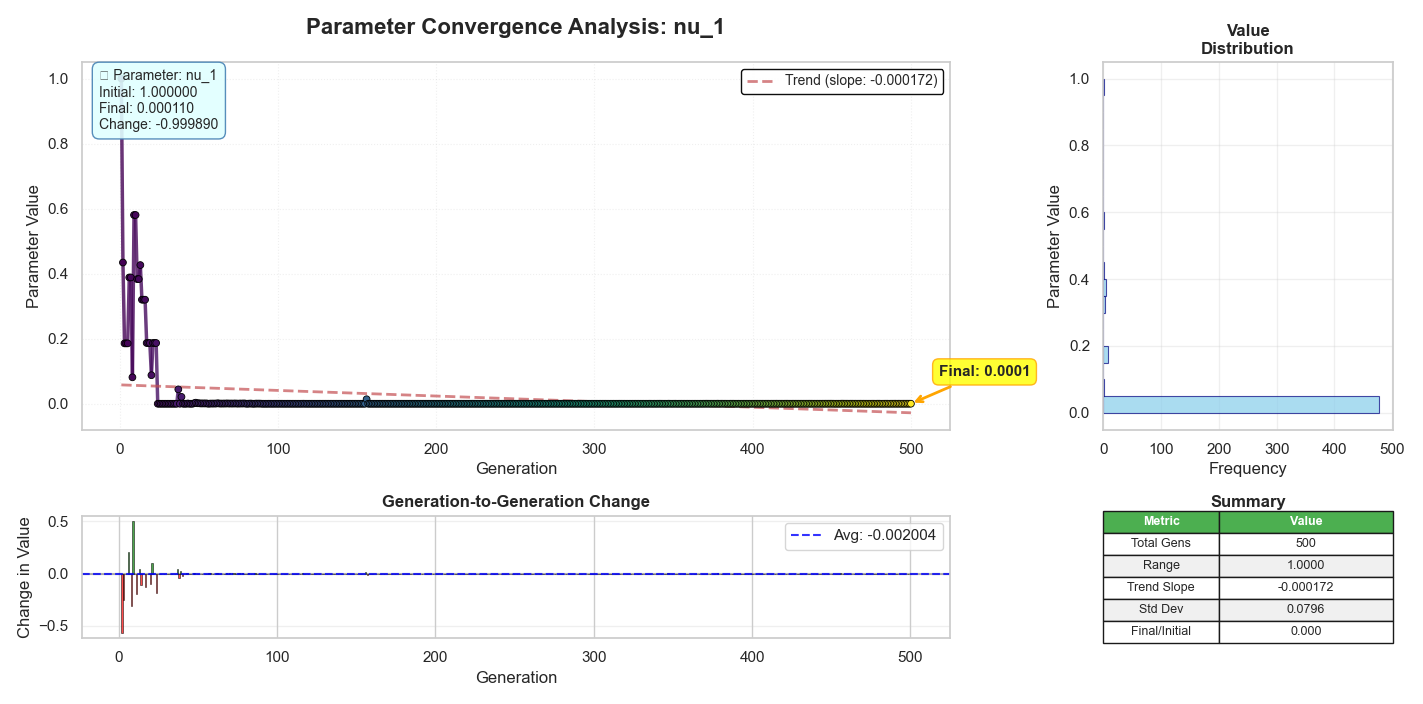
\includegraphics[width=\linewidth]{picture22.png}%
  \caption{همگراییِ پارامترهای \(\nu\): (a) \(\nu_1\).}
  \label{fig:nu_convergence}
\end{figure}

\begin{figure}[h]\ContinuedFloat
  \centering
  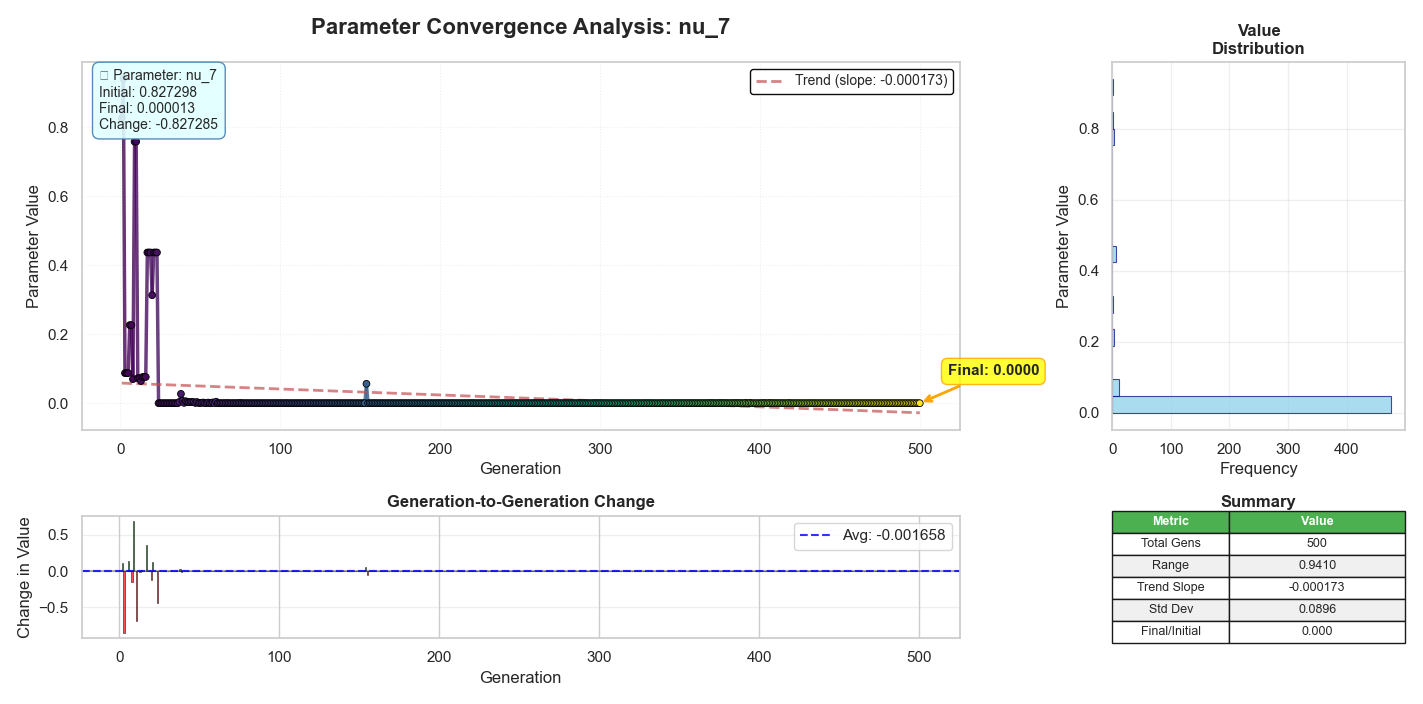
\includegraphics[width=\linewidth]{picture23.png}%
  \caption{(b) \(\nu_7\).}
\end{figure}

\begin{figure}[h]\ContinuedFloat
  \centering
  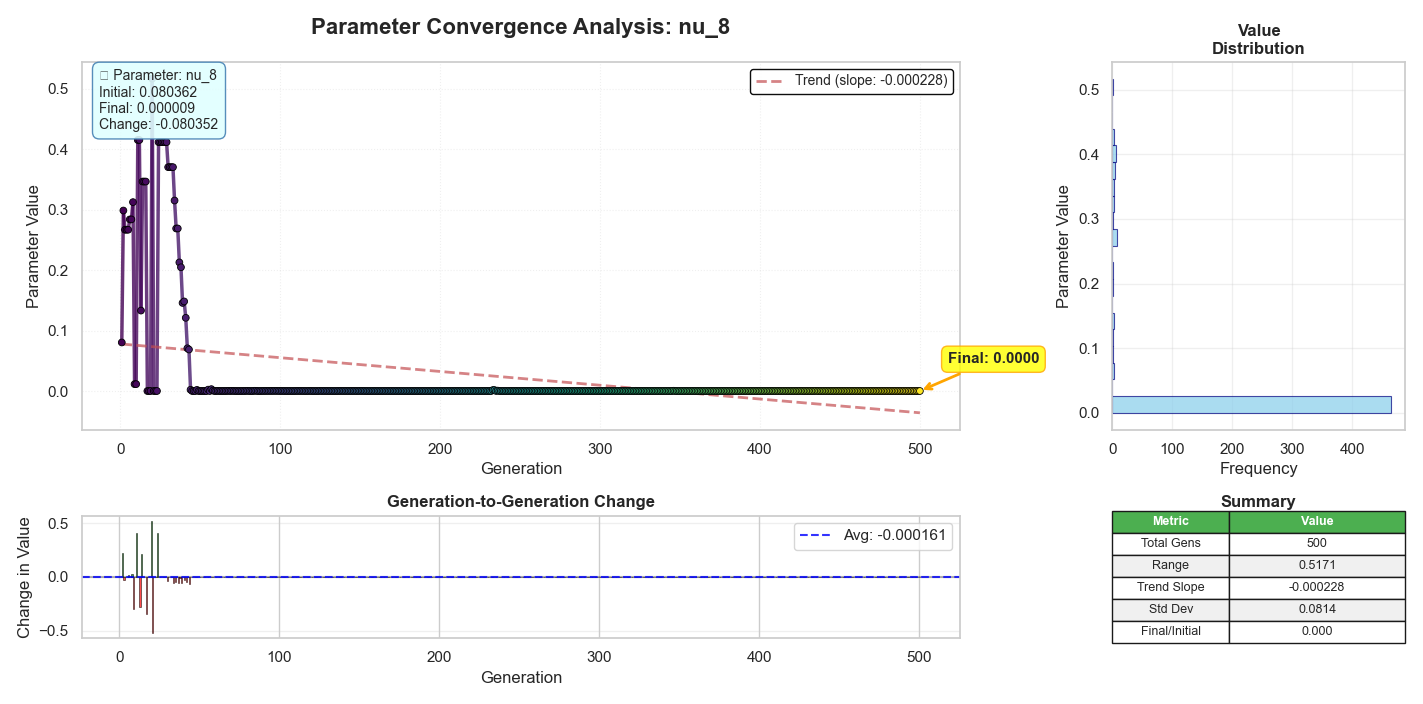
\includegraphics[width=\linewidth]{picture24.png}%
  \caption{(c) \(\nu_8\).}
\end{figure}

\paragraph{تحليل پارامترهاي $\nu$ در شكل‌هاي \ref{fig:nu_convergence}(a)–(c)}
در شكل‌هاي \ref{fig:nu_convergence}(a)، \ref{fig:nu_convergence}(b) و \ref{fig:nu_convergence}(c)، همگراييِ $\nu_1$، $\nu_7$ و $\nu_8$ در بازه‌اي به طول $500$ نسل گزارش شده است. مقادير آغازين به‌ترتيب $1.000000$، $0.827298$ و $0.080362$ ثبت شده و مقادير نهاييِ متناظر $0.000110$، $0.000013$ و $0.000009$ به‌دست آمده است؛ كاهشِ خالص به‌ترتيب $0.999890$، $0.827285$ و $0.080353$ مي‌باشد. گستره‌هاي مشاهده‌شده براي $\nu_1$، $\nu_7$ و $\nu_8$ به‌ترتيب $1.0000$، $0.9410$ و $0.5171$ و انحراف‌معيارها $0.0796$، $0.0896$ و $0.0814$ گزارش شده است. خطوطِ روندِ خطي با شيب‌هاي $-1.72\times 10^{-4}$، $-1.73\times 10^{-4}$ و $-2.28\times 10^{-4}$ به‌ازاي هر نسل برازش داده شده‌اند و ميانگينِ تغييراتِ نسل‌به‌نسل به‌ترتيب $-2.004\times 10^{-3}$، $-1.658\times 10^{-3}$ و $-1.61\times 10^{-4}$ اندازه‌گيري شده است. در هر پنل، پله‌هاي نزوليِ بزرگ در ابتداي اجرا در نمودارِ افزايش‌ها ديده مي‌شود و در ادامه تغييرات در نزديكيِ صفر خوشه‌بندي مي‌شوند. هيستوگرامِ مقادير عمدتاً در كمترينِ بين متمركز است و سكوي‌هاي طولانيِ نزديك به صفر در مسيرها مشاهده مي‌شود. در مجموع، اين الگوها نشان مي‌دهند كه پارامترهاي $\nu$ به‌صورت منسجم به سمتِ بي‌اثري رانده شده و عملاً توسط بهينه‌سازي هرس شده‌اند؛ اين رفتار با هدفِ تنكي و كاهشِ تعدادِ پارامترهايِ فعال \lr{DVA} سازگار است. خلاصه‌ي همگراييِ پارامتر-به-پارامتر در جدول~\ref{tab:conv_summary} ارائه شده است.



\begin{table}[htbp]
\centering
\caption{خلاصه همگراییِ همه پارامترهای تنظیم‌شده در \(500\) نسل}
\label{tab:conv_summary}
\scriptsize
\setlength{\tabcolsep}{3.5pt}
\renewcommand{\arraystretch}{1.25}
\begin{tabular}{c c c c c c c c p{0.38\textwidth}}
\toprule
\textbf{پارامتر} & \textbf{آغازین} & \textbf{نهایی} & $\Delta$ & \textbf{شیبِ روند} & \textbf{میانگین \(\Delta\)/نسل} & \textbf{گستره} & \lr{SD} & \textbf{نتیجه همگرایی} \\
\midrule
\(\beta_1\) & $0.029003$ & $0.015239$ & $-0.013764$ & $-6.0\times 10^{-6}$ & $-2.8\times 10^{-5}$ & $0.0307$ & $0.0028$ & پایدار درونی؛ به‌عنوان تنظیم‌گرِ کوچکِ فعال باقی ماند \\
\(\beta_7\) & $0.591281$ & $0.550909$ & $-0.040372$ & $-4.75\times 10^{-4}$ & $-8.1\times 10^{-5}$ & $0.3503$ & $0.0712$ & پایدار درونی؛ نقشِ غالب در پاسخ \\
\(\beta_8\) & $0.771658$ & $0.000106$ & $-0.771553$ & $-2.93\times 10^{-4}$ & $-1.546\times 10^{-3}$ & $0.7717$ & $0.0621$ & نزدیکِ صفر رانده شد؛ عملاً هرس شد \\
\(\lambda_1\) & $0.772152$ & $0.823493$ & $+0.051342$ & $-1.47\times 10^{-4}$ & $+1.03\times 10^{-4}$ & $0.1695$ & $0.0257$ & پایدار درونی؛ پارامترِ فعال باقی ماند \\
\(\lambda_7\) & $0.388707$ & $0.257990$ & $-0.130717$ & $-4.43\times 10^{-4}$ & $-2.62\times 10^{-4}$ & $0.3565$ & $0.0719$ & پایدار درونی؛ بدونِ رسیدن به کران‌ها مؤثر بود \\
\(\lambda_8\) & $0.948500$ & $0.078876$ & $-0.869625$ & $-6.04\times 10^{-4}$ & $-1.743\times 10^{-3}$ & $0.9110$ & $0.0993$ & به مقدارِ کوچک کاهش یافت؛ اثرگذاری کم‌وزن شد \\
\(\mu_1\) & $0.393887$ & $0.367100$ & $-0.026756$ & $-3.41\times 10^{-4}$ & $-5.4\times 10^{-5}$ & $0.2159$ & $0.0535$ & کاهشِ تدریجی و پایدارسازیِ درونی \\
\(\nu_1\) & $1.000000$ & $0.000110$ & $-0.999890$ & $-1.72\times 10^{-4}$ & $-2.004\times 10^{-3}$ & $1.0000$ & $0.0796$ & فروپاشی به صفر؛ هرس‌شده توسط تنکی \\
\(\nu_7\) & $0.827298$ & $0.000013$ & $-0.827285$ & $-1.73\times 10^{-4}$ & $-1.658\times 10^{-3}$ & $0.9410$ & $0.0896$ & فروپاشی به صفر؛ هرس‌شده توسط تنکی \\
\(\nu_8\) & $0.080362$ & $0.000009$ & $-0.080353$ & $-2.28\times 10^{-4}$ & $-1.61\times 10^{-4}$ & $0.5171$ & $0.0814$ & فروپاشی به صفر؛ هرس‌شده توسط تنکی \\
\bottomrule
\end{tabular}
\end{table}

\section{جمع‌بندي}

\noindent براي دگرگون كردن پاسخ سازه ميزبان در \lr{FRF}، \lr{DVA}‌ها ادوات پسيـوي‌اند كه به سازه ميزبان متصل مي‌شوند. كارايي آن‌ها به چيدمان و تنظيم جرم‌ها، فنرها، ميراگرها و \lr{inerter}‌ها وابسته است؛ تركيبي كه فضاي طراحي پرابعاد و غالباً نا‌محدب پديد مي‌آورد. در رويه‌هاي مرسوم، يك شكاف شناسايي شد: معيار تك‌مقياسيِ قابل تنظيم براي ديكته كردن شكل \lr{FRF} وجود نداشت؛ از تعيينِ جايگاه قله‌ها و پهناي باندِ اجتناب گرفته تا دامنه قله‌ها و شاخص‌هاي مشابه. نتيجه آن بود كه طراحي‌ها بيش از نياز، از مؤلفه‌ها و متغيرهاي تنظيم بهره مي‌گرفتند؛ چرا كه چارچوب‌هاي بهينه‌سازي به ندرت از پيچيدگي غيرضروري مي‌كاستند.

\noindent براي رفع اين نياز، هدف اصلي تعريف يك مقياس امتيازي واحد به نام \emph{معيار تكين} \(C_s\) بود. در ساخت اين مقياس، سنجه‌هاي عملكرد ابتدا نرمال مي‌شوند و سپس با وزن‌هايي كه مستقيماً توسط كاربر انتخاب مي‌گردند تركيب مي‌شوند. امتياز برازندگي از سه جزء تشكيل مي‌شود: جزء انحرافِ \(C_s\) كه \lr{FRF} را به سمت اهداف اعلام‌شده مي‌كشاند؛ جزء خطاي هدف كه ميزان نزديكي پاسخِ حاصل به اهداف را مي‌سنجد؛ و جريمه تنكي كه پارامترهاي غيرضروري را مي‌كاهد و طرح‌هاي ساده را ترجيح مي‌دهد.

\noindent سپس از يك \lr{GA} براي جست‌وجوي فضاي طراحي و يافتن راه‌حل بهينه براي تابع برازندگي استفاده شد. مدل‌سازي، تحليل \lr{FRF}، بهينه‌سازي و پس‌پردازش تا سقف پنج درجه آزادي در نرم‌افزار \lr{DeVana} (توسعه دهي نويسندگان) يكپارچه شد و كل جريان كار با آن پياده‌سازي گرديد. روش‌شناسي با يك بنچمارك كاملاً كوپل \lr{1DOF–1DOF} ارزيابي شد؛ در اين بنچمارك، سامانه اصلي و جذب‌كننده هر دو به دو پايه متحرك از طريق فنر، ميراگر و \lr{inerter} متصل بودند. بازه \(1000\)\,\lr{Hz} تا \(2000\)\,\lr{Hz} به عنوان باندِ اجتناب تعيين شد؛ پاسخِ درون باند توسط \lr{DVA} بهينه سركوب گرديد و دو قله باريك در نزديكي لبه‌هاي باند شكل گرفت. پاسخِ خارج از باند نزديك به خط مبنا باقي ماند. تاريخچه‌هاي برازندگي بهبود سريع ابتدايي را نشان دادند و سپس در مقاديري نزديك به تلرانس همگرايي پايدار شدند. با تفكيك برازندگي به مؤلفه‌ها، روشن شد كنترل جايگاه قله و پهناي باند محقق شده و جزء تنكي مانع تنظيم‌هاي زائد گرديده است. تحليل همگراييِ تك‌تك پارامترها نشان داد تنها زيرمجموعه‌اي كوچك در نقطه بهينه فعال باقي مي‌ماند: همه پارامترهاي \(\nu\) به مقادير نزديك صفر رسيدند و عملاً هرس شدند؛ \(\beta_1\)، \(\beta_7\)، \(\mu_1\)، \(\lambda_1\) و \(\lambda_7\) در نقاط دروني پايدار شدند كه نشانگر وجود بهينه قابل شناسايي (نه رفتارِ محدودشده به مرز) است؛ و \(\beta_8\) و \(\lambda_8\) به مقادير كوچك فروكاستند كه با هدف جلوگيري از استفاده بيش از حد از مؤلفه‌هاي جذب‌كننده سازگار است.

\noindent پيامدهاي كاربردي چندي از اين چارچوب حاصل مي‌شود. نخست، \(C_s\) روشي مستقيم و قابل تفسير براي كُدگذاري نيتِ طراحي فراهم مي‌كند: اهدافِ مربوط به دامنه قله‌ها، جايگاه قله‌ها و پهناي باند را مي‌توان به‌صراحت بيان كرد و بهينه‌ساز آن‌ها را برآورده مي‌كند. دوم، گنجاندن تنكي در تابع هدف به راه‌حل‌هاي كم‌پيچيدگي مي‌انجامد؛ امري كه جرم، هزينه و نگهداشت را كاهش مي‌دهد و حساسيت نسبت به \lr{detuning} و تولرانس‌هاي ساخت را كم مي‌كند. سوم، \lr{GA} بدون بازتنظيمِ دستيِ پارامترهاي الگوريتمي همگراييِ پايدار ارائه داد و به كارگيري در سامانه‌هاي جديد را ساده كرد. چهارم، پياده‌سازي در \lr{DeVana} مسير تكرارپذيري از تعريفِ مدل تا مشخصات سخت‌افزاريِ تنظيم‌شده فراهم مي‌كند و امكان مطالعه‌هاي \lr{what-if} سريع را در خانواده‌هاي جذب‌كننده — از جمله چيدمان‌هاي تقويت‌شده با \lr{inerter} — ميسر مي‌سازد.

\noindent در جمع‌بندي، چارچوبي يكپارچه براي طراحي \lr{DVA} ارائه شد كه معيارِ تكينِ قابل تنظيم و نرمال‌شده را با يك \lr{GA} تطبيقي در محيط \lr{DeVana} تركيب مي‌كند. اين رويكرد، شكل‌دهي مستقيم \lr{FRF} را ممكن مي‌سازد و هم‌زمان از افراط در تعداد پارامترهاي جذب‌كننده جلوگيري مي‌كند. مطالعه بنچمارك نشان داد كه باندِ اجتنابِ مشخص قابل حفاظت است و طرح نهايي تنك و قابل تفسير باقي مي‌ماند. اين نتايج پايه‌اي عملي براي طراحيِ كارآمدِ جذب‌كننده‌هاي هدف‌محور فراهم مي‌كند و مسير روشني به سمت راه‌حل‌هاي مقاوم، بلادرنگ و قابل راستي‌آزماييِ تجربي مي‌گشايد.





